\documentclass[a4paper, oneside]{book}
\usepackage{tikz, hyperref}
\hypersetup{
	colorlinks=true,
	urlcolor=blue,
	linkcolor=black
	}

\title{Alchemy University}
\author{0xdorifto}
\date{February, 2023}

\begin{document}

\maketitle

\tableofcontents

%CHAPTER 1
\chapter{Blockchain Cryptography}

\section{Bootcamp Introduction}

\subsection{Tips and Tricks}

Some tips for the bootcamp.

\section{The First Primitive}

\subsection{Blockchain and Crypto}

\begin{itemize}
	\item The purpose of the Blockchain is to have a network of computers agree upon a common state of data, A.K.A. \underline{reach consensus}.
	\item Most common use of Blockchain is \underline{cryptocurrency}.
	\item Bitcoin is a public ledger of transactions.
	\item The problem with a private ledger is that you need to underline{trust} the owner to not tamper with it.
	\item The difference between a \underline{smart contract} and a regular piece of code is that it is publically available and enforced through financial incentives.
	\item An \underline{hash functions} takes an input of any size and turn it into a fixed size output.
	\item A \underline{cryptographic hash function} has 5 characteristics 
	\begin{itemize}
		\item Deterministic
		\item Pseudo random
		\item One-way
		\item Fast to Compute
		\item Collision Resistant
	\end{itemize}
	\item Blockchains store inputs by storing it's hash output.
	\item The blockchain consensus mechanism is \underline{proof of work}.
\end{itemize}

\subsection{Cryptographic Hashes}

\textsf{Problem:} Given a SHA256 hash, find the color input that would generate that hash. You can assume that all the hashes be generated only from colors provided in the COLORS array.

\noindent \textsf{Solution:}

\begin{verbatim}
const { sha256 } = require("ethereum-cryptography/sha256");
const { toHex, utf8ToBytes } = require("ethereum-cryptography/utils");

// the possible colors that the hash could represent
const COLORS = ['red', 'green', 'blue', 'yellow', 'pink', 'orange'];

// given a hash, return the color that created the hash'
function findColor(hash) {
    return COLORS.find(x => toHex(sha256(utf8ToBytes(x))) === toHex(hash));
}

module.exports = findColor;
\end{verbatim}

\section{Digital Signatures}
\subsection{Public Key Cryptography}
\begin{itemize}
	\item \underline{Cryptography} is the study of encrypting messages.
	\item \underline{Symmetric key Cryptography} is when multiple parties have the same key to decrypt messages.
	\item With the above, the function to encrypt and to decrypt a message is the same.
	\item The problem with this is that you have to have met the other parties before to share the key.
	\item \underline{Public key cryptography} A.K.A underline{Asymetric Cryptography} solves this issue.
	\item The owner of the private key can prove he is the author of the message because only he has the private key.
	
	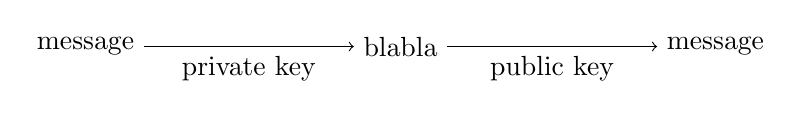
\begin{tikzpicture}
		\node at (0,0) (A) {message};
		\node at (4,0) (B) {blabla};
		\node at (8,0) (C) {message};
		
		\draw [->] (A) -- node[anchor=north] {private key} (B);
		\draw [->] (B) -- node[anchor=north] {public key} (C);
	\end{tikzpicture}
	
	\item Anyone can send him a secure message that only he can read, because only he has the private key.
	
	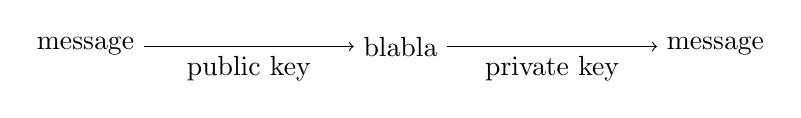
\begin{tikzpicture}
		\node at (0,0) (A) {message};
		\node at (4,0) (B) {blabla};
		\node at (8,0) (C) {message};
		
		\draw [->] (A) -- node[anchor=north] {public key} (B);
		\draw [->] (B) -- node[anchor=north] {private key} (C);
	\end{tikzpicture}
	
	\item \underline{RSA} is a public key cryptography algorithm that works with prime numbers.
	\item \underline{ECDSA} is a public key cryptography algorithm that works with elliptic curves. It is the one used by BTC.
	\item Addresses are generated from the public key.
\end{itemize}

\subsection{Public Key Exercise}

\subsection{Further Study}

\begin{itemize}
	\item ECDSA
	\begin{itemize}
		\item \href{https://blog.cloudflare.com/ecdsa-the-digital-signature-algorithm-of-a-better-internet/}{Cloudfare: ECDSA: The digital signature algorithm of a better internet}
		\item \href{https://en.wikipedia.org/wiki/Elliptic_Curve_Digital_Signature_Algorithm}{Wikipedia: Elliptic Curve Digital Signature Algorithm}
		\item \href{https://cryptobook.nakov.com/digital-signatures/ecdsa-sign-verify-messages}{PCD: ECDSA: Elliptic Curve Signatures}
	\end{itemize}
	\item Bitcoin
	\begin{itemize}
		\item \href{https://en.bitcoin.it/wiki/Secp256k1}{Bitcoin Wiki: Secp256k1}
		\item \href{https://en.bitcoin.it/wiki/Invoice_address}{Bitcoin Wiki: Invoice address}
		\item \href{https://en.bitcoin.it/wiki/Technical_background_of_version_1_Bitcoin_addresses}{Bitcoin Wiki: Technical background of version 1 Bitcoin addresses}
		\item \href {https://bitcoin.org/bitcoin.pdf}{Bitcoin Whitepaper}
	\end{itemize}
	\item Diffie-Hellman Key Exchange
	\begin{itemize}
		\item \href{https://en.wikipedia.org/wiki/Diffie%E2%80%93Hellman_key_exchange}{Wikipedia: Diffie–Hellman key exchange}
		\item \href{https://security.stackexchange.com/questions/41205/diffie-hellman-and-its-tls-ssl-usage/41226#41226}{Stack Exchange: Diffie-Hellman and its TLS/SSL usage}
	\end{itemize}
	\item RSA
	\begin{itemize}
		\item \href{https://en.wikipedia.org/wiki/RSA_(cryptosystem)}{Wikipedia: RSA (cryptosystem)}
		\item \href{https://cryptobook.nakov.com/digital-signatures/rsa-signatures}{PCD: RSA Signatures}
		\item \href{https://www.youtube.com/watch?v=4zahvcJ9glg}{Eddie Woo: The RSA Encryption Algorithm (1 of 2: Computing an Example)}
		\item \href{https://www.youtube.com/watch?v=oOcTVTpUsPQ}{Eddie Woo: The RSA Encryption Algorithm (2 of 2: Generating the Keys)}
		\item \href{https://www.reuters.com/article/us-usa-security-nsa-rsa/exclusive-nsa-infiltrated-rsa-security-more-deeply-than-thought-study-idUSBREA2U0TY20140331}{Reuters: Exclusive: NSA infiltrated RSA security more deeply than thought - study}
	\end{itemize}
\end{itemize}

\section{Proof of Work}
\subsection{Mining and Proof-of-Work}

\subsection{Proof of Work Miner}

\subsection{Proof of Work}

\subsection{Further Study}

\section{Blockchain Network}
\subsection{Blockchain Structure}
\subsection{Blockchain Data Structure}
\subsection{Further Study}

\section{Project}
\subsection{ECDSA Node}


%CHAPTER 2
\chapter{Blockchain Storage}

\section{Keeping Track of Blockchain User State}
\subsection{UTXO vs Account Model}
\subsection{Coding the UTXO Model}
\subsection{UTXO Locking and Unlocking Scripts}

\section{Tree Data Structure}
\subsection{Basic Tree Data Structures}
\subsection{Build a Binary Search Tree}
\subsection{Merkle Tree Into}
\subsection{Merkle Trees}

\section{Blockchain Data Storage}
\subsection{Merkle Trees in Blockchains}
\subsection{Ethereum Tries}
\subsection{Learn Tries}
\subsection{Supplemental Reading}

\section{Assignments}
\subsection{Merkle Gift List}


%CHAPTER 3
\chapter{Ethereum}

\section{Ethereum Features}
\subsection{Introduction to Ethereum}
\subsection{Proof of Stake}
\subsection{Gas on Ethereum}
\subsection{Transaction Game}
\subsection{Ethereum Accounts}
\subsection{Supplemental Reading}

\section{Reading Data from Ethereum}
\subsection{Read Requests}
\subsection{Activity: Query Ethereum}
\subsection{Ethereum Nodes}
\subsection{JSON-RPC Requests}

\section{Ethereum Transactions}
\subsection{Ethereum Nodes}
\subsection{JSON-RPC Requests}

\section{Front-End Libraries}
\subsection{Intro to Front-end Libraries}
\subsection{Intro to Ether.js}
\subsection{Where is the Ether?}

\section{Assignments}
\subsection{Build your own Block Explorer}


%CHAPTER 4
\chapter{Smart Contract Basics}

\section{Solidity Syntax}
\subsection{Solidity Syntax}
\subsection{Data Types}
\subsection{Solidity and the EVM}
\subsection{Solidity at a Glance}

\section{Functions}
\subsection{Solidity Functions}
\subsection{Functions}

\section{Smart Contract Communication}
\subsection{Contract Communication}
\subsection{Contract with ethers.js}

\section{Intro to Hardhat}
\subsection{What is Hardhat?}
\subsection{Guide: How to Deploy a Contract with Ethers + Hardhat}
\subsection{Guide: How to Modify State using Hardhat}

\section{Address Interactions}
\subsection{Calling EOAs}
\subsection{Sending Ether}
\subsection{Reverting Transactions}
\subsection{Learning Revert}
\subsection{Calling Contracts}
\subsection{Sending Data}

\section{Practice Solidity}
\subsection{Sum and Average}
\subsection{Countdown}

\section{Assignments}
\subsection{Smart Contract Winner}
\subsection{Hardhat Guide: How To Unit Test Contracts}
\subsection{Week 4 Recap + Feedback}


%CHAPTER 5
\chapter{Solidity}

\section{Mappings}
\subsection{Mappings}
\subsection{Mappings}
\subsection{Contract Puzzles}

\section{Events}
\subsection{Events}
\subsection{Local Hardhat Games}
\subsection{Events}

\section{Escrow Contract}
\subsection{Escrow Introduction}
\subsection{Build an Escrow}

\section{Reference Types}
\subsection{Arrays and Structs}
\subsection{Arrays}
\subsection{Structs}

\section{Project}
\subsection{Decentralized Escrow Application}

%CHAPTER 6
\chapter{Solidity Core}

\section{Solidity Challenges}
\subsection{Solidity Practice}
\subsection{Party Split}
\subsection{Dead Man's Switch}
\subsection{Hackathon Ratings}

\section{Multi-Sigs}
\subsection{What is a Multi-Sig Contract?}
\subsection{Multiple Signature Wallet}

\section{Inheritance}
\subsection{What is Inheritance?}
\subsection{Inheritance}

\section{ERC-20}
\subsection{What is the ERC-20 Token Standard?}
\subsection{ERC-20 Token}
\subsection{Deploy Your Own Token}
\subsection{ERC-20 Treasure Chest}
\subsection{Send ERC-20s to Contracts}
\subsection{ERC-20 Token Indexer App}

\section{NFTs}
\subsection{What Are NFTs?}
\subsection{How to Mint NFTs}
\subsection{NFT Indexer App}

\section{Recap}
\subsection{Recap}


%CHAPTER 7
\chapter{Solidity Governance}


\section{Proxy Contracts}
\subsection{Storage Slots}
\subsection{Delefatecall}
\subsection{Evolution of Proxies}

\section{Libraries}
\subsection{Introduction to Libraries}
\subsection{Smart Contract Libraries}

\section{Upgrading Contracts}
\subsection{What is Smart Contract Upgradeability?}
\subsection{Deploy Upgradeable Smart Contracts}

\section{Governance}
\subsection{The State of Governance}
\subsection{Basic Governace}
\subsection{The Governor Standard}

\section{Recap}
\subsection{Recap}


%CHAPTER 8
\chapter{Final Project and Certifications}

\section{Final Project}
\subsection{Final Project Guidelines}
\subsection{Final Project Resources}
\subsection{Final Project Submission}

\end{document}

